\documentclass[12pt,letterpaper]{article}
\usepackage{amsmath,amsthm,amsfonts,amssymb,amscd}
\usepackage{listings}
\usepackage{hyperref}
\usepackage{graphicx}
\usepackage{enumerate}
\usepackage{fancyhdr}
\usepackage{mathrsfs}
\usepackage[margin=3cm]{geometry}
\setlength{\parindent}{0.0in}
\setlength{\parskip}{0.05in}

% Edit these as appropriate
\newcommand\course{CS595}
\newcommand\semester{FAll 2013}     
\newcommand\hwnum{2}
\newcommand\yourname{Mohamed Aturban}
\newcommand\login{maturban}

\newenvironment{answer}[1]{
  \subsubsection*{Problem #1}
}

\pagestyle{fancyplain}
\headheight 35pt
\lhead{\yourname\ (\login)\\\course\ --- \semester}
\chead{\textbf{\Large Assignment \hwnum}}
\rhead{\today}
\headsep 10pt

\begin{document}

\begin{answer}{1}
To search for links within tweets in my twitter account maturban1, I have used exactly the same way suggested in problem 1 in our assignment:
\url{http://thomassileo.com/blog/2013/01/25/using-twitter-rest-api-v1-dot-1-with-python/}
 List of key words, around 70, is used for the search. The idea is that the program will start searching the first word, collect possible links, and then continue searching the second work and so on. It stops either if collecting 1000 URIs or there is no more key words. In order to approve a link and add it to a final list, its effective url must be checked for the following:

\begin{itemize}
\item HTML code 200
\item It is not already in the final list
\item Content type 'text/html'
\item It does not belong to "instagram.com" because, at the beginning,  I got around 95 percent of links belong to this website!
\item If the URI is split around '/'. the last part of the URI must contains one of the special characters or a white space. 
\end{itemize}

The program will store the results in a file called "twitterLinks.txt", the result could be something like:

\begin{figure}[ht!]
\centering
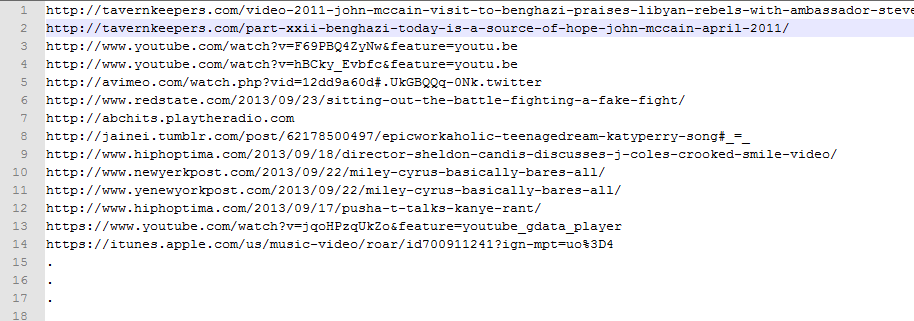
\includegraphics[scale=0.75]{links11}
\caption{Output URIs}
\label{overflow}
\end{figure}

"getTwitterLinks.py" contains Python code for solving problem 1. "links.txt" is the output file.


\end{answer}

\begin{answer}{2}

Curl is used within Python to get number of mementos for each URI. The Curl command looks like:
\begin{lstlisting}[language=bash]
$curl http://mementoproxy.cs.odu.edu/aggr/timemap/link/[link is here]
\end{lstlisting}
Because some of the returned lines should not be counted as a memento, only lines that have the key word "datetime=" will do. Unfortunately. The following histogram illustrates that most of the URIs come with Zero memento:

 \begin{figure}[ht!]
\centering
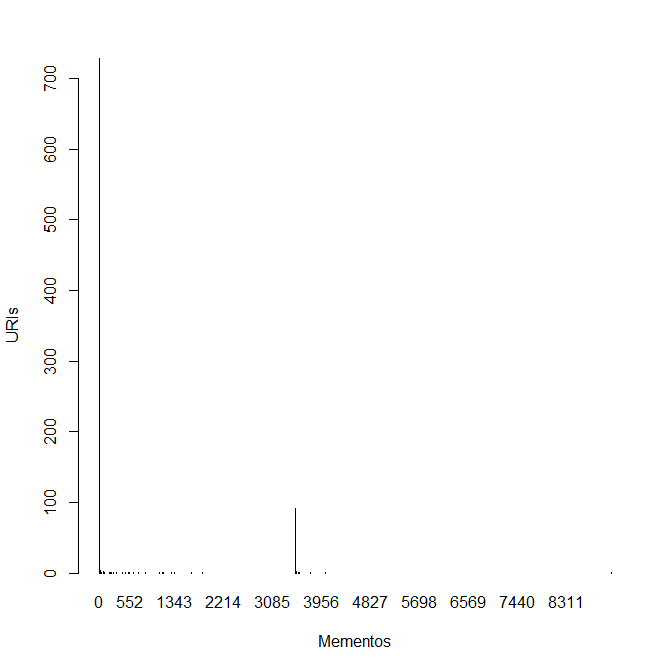
\includegraphics[scale=0.75]{memento}
\caption{Mementos vs URIs}
\label{overflow}
\end{figure}

"getMementos.py" contains Python code for solving problem 2. "mementos.txt" is the output file.

\end{answer}

\begin{answer}{3}

Carbon Date tool is installed and used to estimate the age of the 1000 URIs. Also, Curl within Python code is used to connect the Carbon Date server, and because it takes time, several minutes, for the server to respond and send back results, five copies of this tool are run in parallel. This will help to finish estimating the 1000 URIs age more fast. The following plot shows how the number of mementos is effected by the age of the URIs. Only URIs that have mementos are included in this chart. Two URIs with age (0 days) are included in the plot also. I did not remove them because (0 days) indicates that the age of these URIs is less than 24 hours.


\begin{figure}[ht!]
\centering
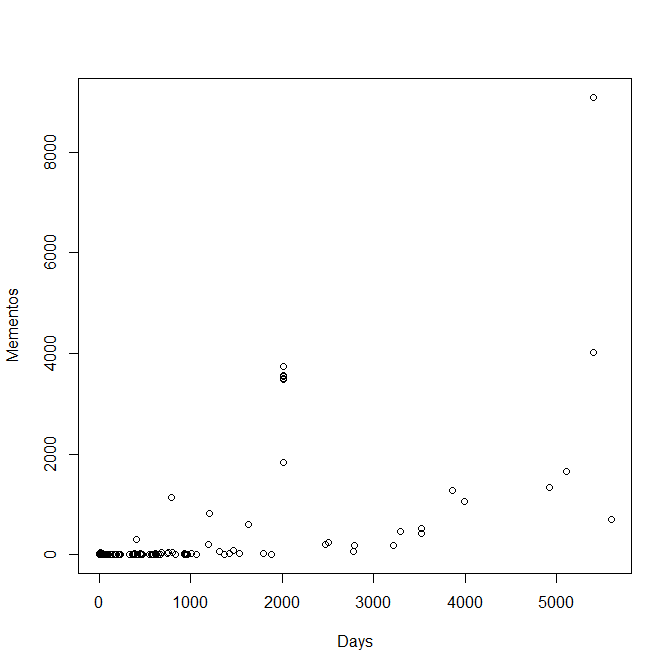
\includegraphics[scale=0.75]{URI}
\caption{URIs age (in Days) vs Mementos}
\label{overflow}
\end{figure}


The plot shows that the young URIs get less chance of having more mementos! Finally, I would like to indicate that R language is used for plotting. I am still new in this environment. Next, I will try to understand how to use good scale to represent data more clear in plots. 

"getURIAge.py" contains Python code for solving problem 3. "age.txt" is the output file.

\end{answer}

\end{document}
